\documentclass[11pt]{article}
\usepackage{../../styles/activity}

\usepackage{xr}
\externaldocument{0-MR}

\lhead{}
%\chead{\textbf{\Large{\hspace{0pt}Beginning Activities for Section~6.6}}\\\hspace{0pt}\emph{Mathematical Reasoning: Writing and Proof}}
\bahead{6.6}
\rhead{}
\lfoot{}
\rfoot{}
\cfoot{\hspace{0pt}\scalebox{0.4}{
\includegraphics{cc-by-nc-sa.eps}}}

\begin{document}
\subsection*{Beginning Activity 1 (Functions and Sets)}
Each set in this beginning activity is described using set builder notation and the roster method.  This is frequently done.  Please notice the correct use the equality sign when this done.
\begin{enumerate}
\begin{multicols}{2}
\item \begin{enumerate}
\item $\left\{ f \left( x \right) \mid x \in A \right\} = \left\{ s, t \right\}$

\item $\left\{ f \left( x \right) \mid x \in B \right\} = \left\{ s \right\}$
\end{enumerate}

\item \begin{enumerate}
\item $\left\{ x \in S \mid f \left( x \right) \in C \right\} = \left\{ a, b, c, d \right\}$

\item $\left\{ x \in S \mid f \left( x \right) \in D \right\} = \left\{ a, d \right\}$
\end{enumerate}
\end{multicols}
%



%\begin{enumerate}
%\item \begin{multicols}{4}
%$f \left( 1 \right) = 1$
%
%$f \left( 2 \right) = 4$
%
%$f \left( 3 \right) = 9$
%
%$f \left( -1 \right) = 1$
\item $\left\{ f \left( x \right) \mid x \in A \right\} = \left\{ 1, 4, 9 \right\}$

\item \begin{enumerate}
\item $\left\{ x \in \R \mid g\left( x \right) = 1 \right\} = \left\{ -1, 1 \right\}$.
\item $\left\{ x \in \R \mid g\left( x \right) = 9 \right\} = \left\{ -3, 3 \right\}$.
\item $\left\{ x \in \R \mid f\left( x \right) = 15 \right\} = \left\{ -\sqrt{15}, \sqrt{15} \right\}$.

\item There are no $x \in \mathbb{R}$ such that $g \left( x \right) = -1$, and so,
$\left\{ x \in \R \mid g\left( x \right) = -1 \right\} = \emptyset$.
\end{enumerate}

\item For each element $y$ in the set $B$, we must determine all $x \in \R$ such that $g(x) = y$.  For example, $9 \in B$, and if we solve $g(x) = 9$, where $x \in \R$, we get $x = -3$ or $x = 3$.

$\left\{ x \in \mathbb{R} \mid g \left( x \right) \in B \right\} = \left\{ -1, 1, -3, 3, 
-\sqrt{15}, \sqrt{15} \right\}$

\end{enumerate}
\hbreak%


\newpage
\subsection*{Beginning Activity 2 (Functions and Intervals)} 
\begin{figure}[h]
\begin{center}
\scalebox{0.75}{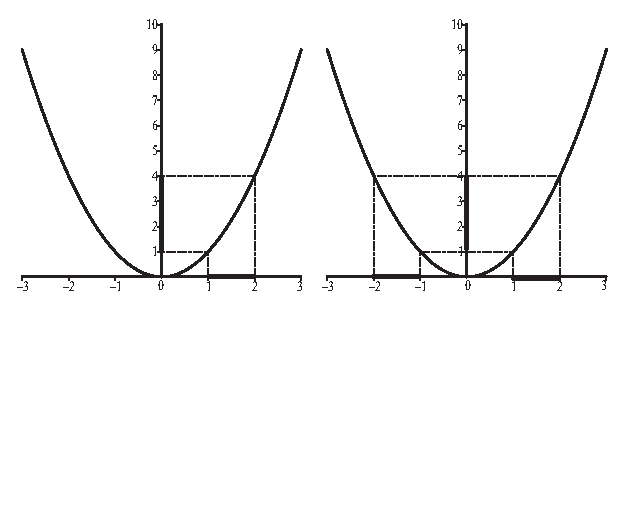
\includegraphics{figps-preview6-6.eps}} 
\caption{Graphs for Beginning Activity 2}
\end{center}
\end{figure}
\begin{enumerate}
\item \begin{enumerate} \setcounter{enumii}{2}
\item $\left\{ f \left( x \right) \mid x \in \left[ 1, 2 \right] \right\} = 
\left\{ x \in \mathbb{R} \mid 1 \leq x \leq 4 \right\}$.  That is, 
$\left\{ f \left( x \right) \mid x \in \left[ 1, 2 \right] \right\}$ is the closed interval
$\left[ 1, 4 \right]$.
\end{enumerate}

\item \begin{enumerate} \setcounter{enumii}{2}
\item $\begin{aligned}[t]
\left\{ x \in \mathbb{R} \mid f \left( x \right) \in \left[ 1, 4 \right] \right\} &= 
\left\{ x \in \mathbb{R} \mid -2 \leq x \leq -1 \text{ or } 1 \leq x \leq 2 \right\} \\
 &= 
\left\{ x \in \mathbb{R} \mid -2 \leq x \leq -1 \right\} \cup \left\{x \in \mathbb{R} \mid  1 \leq x \leq 2 \right\} \\
&= \left[ -2, -1 \right] \cup \left[ 1, 2 \right]
\end{aligned}$

That is, $\left\{ x \in \mathbb{R} \mid f \left( x \right) \in \left[ 1, 4 \right] \right\}$ is the union of the closed interval $\left[ -2, -1 \right]$ with the closed interval  
$\left[ 1, 2 \right]$.
\end{enumerate}

\hbreak


\end{enumerate}




\end{document}
